\documentclass[twoside]{book}

% Packages required by doxygen
\usepackage{fixltx2e}
\usepackage{calc}
\usepackage{doxygen}
\usepackage[export]{adjustbox} % also loads graphicx
\usepackage{graphicx}
\usepackage[utf8]{inputenc}
\usepackage{makeidx}
\usepackage{multicol}
\usepackage{multirow}
\PassOptionsToPackage{warn}{textcomp}
\usepackage{textcomp}
\usepackage[nointegrals]{wasysym}
\usepackage[table]{xcolor}

% Font selection
\usepackage[T1]{fontenc}
\usepackage[scaled=.90]{helvet}
\usepackage{courier}
\usepackage{amssymb}
\usepackage{sectsty}
\renewcommand{\familydefault}{\sfdefault}
\allsectionsfont{%
  \fontseries{bc}\selectfont%
  \color{darkgray}%
}
\renewcommand{\DoxyLabelFont}{%
  \fontseries{bc}\selectfont%
  \color{darkgray}%
}
\newcommand{\+}{\discretionary{\mbox{\scriptsize$\hookleftarrow$}}{}{}}

% Page & text layout
\usepackage{geometry}
\geometry{%
  a4paper,%
  top=2.5cm,%
  bottom=2.5cm,%
  left=2.5cm,%
  right=2.5cm%
}
\tolerance=750
\hfuzz=15pt
\hbadness=750
\setlength{\emergencystretch}{15pt}
\setlength{\parindent}{0cm}
\setlength{\parskip}{3ex plus 2ex minus 2ex}
\makeatletter
\renewcommand{\paragraph}{%
  \@startsection{paragraph}{4}{0ex}{-1.0ex}{1.0ex}{%
    \normalfont\normalsize\bfseries\SS@parafont%
  }%
}
\renewcommand{\subparagraph}{%
  \@startsection{subparagraph}{5}{0ex}{-1.0ex}{1.0ex}{%
    \normalfont\normalsize\bfseries\SS@subparafont%
  }%
}
\makeatother

% Headers & footers
\usepackage{fancyhdr}
\pagestyle{fancyplain}
\fancyhead[LE]{\fancyplain{}{\bfseries\thepage}}
\fancyhead[CE]{\fancyplain{}{}}
\fancyhead[RE]{\fancyplain{}{\bfseries\leftmark}}
\fancyhead[LO]{\fancyplain{}{\bfseries\rightmark}}
\fancyhead[CO]{\fancyplain{}{}}
\fancyhead[RO]{\fancyplain{}{\bfseries\thepage}}
\fancyfoot[LE]{\fancyplain{}{}}
\fancyfoot[CE]{\fancyplain{}{}}
\fancyfoot[RE]{\fancyplain{}{\bfseries\scriptsize Generated by Doxygen }}
\fancyfoot[LO]{\fancyplain{}{\bfseries\scriptsize Generated by Doxygen }}
\fancyfoot[CO]{\fancyplain{}{}}
\fancyfoot[RO]{\fancyplain{}{}}
\renewcommand{\footrulewidth}{0.4pt}
\renewcommand{\chaptermark}[1]{%
  \markboth{#1}{}%
}
\renewcommand{\sectionmark}[1]{%
  \markright{\thesection\ #1}%
}

% Indices & bibliography
\usepackage{natbib}
\usepackage[titles]{tocloft}
\setcounter{tocdepth}{3}
\setcounter{secnumdepth}{5}
\makeindex

% Hyperlinks (required, but should be loaded last)
\usepackage{ifpdf}
\ifpdf
  \usepackage[pdftex,pagebackref=true]{hyperref}
\else
  \usepackage[ps2pdf,pagebackref=true]{hyperref}
\fi
\hypersetup{%
  colorlinks=true,%
  linkcolor=blue,%
  citecolor=blue,%
  unicode%
}

% Custom commands
\newcommand{\clearemptydoublepage}{%
  \newpage{\pagestyle{empty}\cleardoublepage}%
}

\usepackage{caption}
\captionsetup{labelsep=space,justification=centering,font={bf},singlelinecheck=off,skip=4pt,position=top}

%===== C O N T E N T S =====

\begin{document}

% Titlepage & ToC
\hypersetup{pageanchor=false,
             bookmarksnumbered=true,
             pdfencoding=unicode
            }
\pagenumbering{alph}
\begin{titlepage}
\vspace*{7cm}
\begin{center}%
{\Large Proyecto C\+P\+P2020 }\\
\vspace*{1cm}
{\large Generated by Doxygen 1.8.13}\\
\end{center}
\end{titlepage}
\clearemptydoublepage
\pagenumbering{roman}
\tableofcontents
\clearemptydoublepage
\pagenumbering{arabic}
\hypersetup{pageanchor=true}

%--- Begin generated contents ---
\chapter{Class Index}
\section{Class List}
Here are the classes, structs, unions and interfaces with brief descriptions\+:\begin{DoxyCompactList}
\item\contentsline{section}{\hyperlink{classComplex}{Complex} \\*Clase \hyperlink{classComplex}{Complex} }{\pageref{classComplex}}{}
\item\contentsline{section}{\hyperlink{classDatos}{Datos} \\*Clase \hyperlink{classDatos}{Datos} }{\pageref{classDatos}}{}
\item\contentsline{section}{\hyperlink{classDFT__1d}{D\+F\+T\+\_\+1d} \\*Clase \hyperlink{classDFT__1d}{D\+F\+T\+\_\+1d} }{\pageref{classDFT__1d}}{}
\item\contentsline{section}{\hyperlink{classFFT__1d}{F\+F\+T\+\_\+1d} \\*Clase \hyperlink{classFFT__1d}{F\+F\+T\+\_\+1d} }{\pageref{classFFT__1d}}{}
\end{DoxyCompactList}

\chapter{File Index}
\section{File List}
Here is a list of all documented files with brief descriptions\+:\begin{DoxyCompactList}
\item\contentsline{section}{/home/daniel/\+Escritorio/\+Proyecto/src/apps/\hyperlink{DFT_8cpp}{D\+F\+T.\+cpp} \\*Algoritmo para obtener el tiempo de calculo de D\+FT }{\pageref{DFT_8cpp}}{}
\item\contentsline{section}{/home/daniel/\+Escritorio/\+Proyecto/src/apps/\hyperlink{FFT_8cpp}{F\+F\+T.\+cpp} \\*Algoritmo para obtener el tiempo de calculo de F\+FT }{\pageref{FFT_8cpp}}{}
\item\contentsline{section}{/home/daniel/\+Escritorio/\+Proyecto/src/lib/include/\hyperlink{Complex_8hpp}{Complex.\+hpp} \\*Clase para almacenar datos tipo complejos }{\pageref{Complex_8hpp}}{}
\item\contentsline{section}{/home/daniel/\+Escritorio/\+Proyecto/src/lib/include/\hyperlink{Datos_8hpp}{Datos.\+hpp} \\*Clase para obtener y manipular los datos de entrada para los algoritmos }{\pageref{Datos_8hpp}}{}
\item\contentsline{section}{/home/daniel/\+Escritorio/\+Proyecto/src/lib/include/\hyperlink{DFT__1d_8hpp}{D\+F\+T\+\_\+1d.\+hpp} \\*Clase para calcular la D\+FT }{\pageref{DFT__1d_8hpp}}{}
\item\contentsline{section}{/home/daniel/\+Escritorio/\+Proyecto/src/lib/include/\hyperlink{FFT__1d_8hpp}{F\+F\+T\+\_\+1d.\+hpp} \\*Clase para calcular la F\+FT }{\pageref{FFT__1d_8hpp}}{}
\end{DoxyCompactList}

\chapter{Class Documentation}
\hypertarget{classComplex}{}\section{Complex Class Reference}
\label{classComplex}\index{Complex@{Complex}}


Clase \hyperlink{classComplex}{Complex}.  




{\ttfamily \#include $<$Complex.\+hpp$>$}

\subsection*{Public Attributes}
\begin{DoxyCompactItemize}
\item 
\mbox{\Hypertarget{classComplex_aed0f7f2a72da406620581d863a6dc333}\label{classComplex_aed0f7f2a72da406620581d863a6dc333}} 
double \hyperlink{classComplex_aed0f7f2a72da406620581d863a6dc333}{Re} = 0
\begin{DoxyCompactList}\small\item\em Parte real. \end{DoxyCompactList}\item 
\mbox{\Hypertarget{classComplex_a25938efdb07e8d21e4a07392a3494e0b}\label{classComplex_a25938efdb07e8d21e4a07392a3494e0b}} 
double \hyperlink{classComplex_a25938efdb07e8d21e4a07392a3494e0b}{Im} = 0
\begin{DoxyCompactList}\small\item\em Parte imaginaria. \end{DoxyCompactList}\end{DoxyCompactItemize}


\subsection{Detailed Description}
Clase \hyperlink{classComplex}{Complex}. 

Esta clase contiene dos variables tipo double para representar un numero complejo. 

The documentation for this class was generated from the following file\+:\begin{DoxyCompactItemize}
\item 
/home/daniel/\+Escritorio/\+Proyecto/src/lib/include/\hyperlink{Complex_8hpp}{Complex.\+hpp}\end{DoxyCompactItemize}

\hypertarget{classDatos}{}\section{Datos Class Reference}
\label{classDatos}\index{Datos@{Datos}}


Clase \hyperlink{classDatos}{Datos}.  




{\ttfamily \#include $<$Datos.\+hpp$>$}

\subsection*{Public Member Functions}
\begin{DoxyCompactItemize}
\item 
void \hyperlink{classDatos_ac78505e094f3f4700885bdbc1f606b3f}{obtener\+\_\+datos} (\hyperlink{classComplex}{Complex} $\ast$data, int N)
\begin{DoxyCompactList}\small\item\em Metodo para obtener un array de tamaño N y guardarlo en data. \end{DoxyCompactList}\item 
void \hyperlink{classDatos_a11e17c459622f71bf8c983244668d78e}{bit\+Reversef} (\hyperlink{classComplex}{Complex} $\ast$entrada, \hyperlink{classComplex}{Complex} $\ast$salida, int n, int N)
\begin{DoxyCompactList}\small\item\em Metodo para obtener un array nuevo en orden Bit-\/\+Reversal para el calculo del F\+FT. \end{DoxyCompactList}\item 
double \hyperlink{classDatos_a533dc2344d335ee6b5ac38885442010c}{funcion} (double x, int N)
\begin{DoxyCompactList}\small\item\em Metodo para obtener el valor de una funcion. \end{DoxyCompactList}\end{DoxyCompactItemize}


\subsection{Detailed Description}
Clase \hyperlink{classDatos}{Datos}. 

Esta clase contiene varios metodos para la obtencion y manipulacion de datos. 

\subsection{Member Function Documentation}
\mbox{\Hypertarget{classDatos_a11e17c459622f71bf8c983244668d78e}\label{classDatos_a11e17c459622f71bf8c983244668d78e}} 
\index{Datos@{Datos}!bit\+Reversef@{bit\+Reversef}}
\index{bit\+Reversef@{bit\+Reversef}!Datos@{Datos}}
\subsubsection{\texorpdfstring{bit\+Reversef()}{bitReversef()}}
{\footnotesize\ttfamily void Datos\+::bit\+Reversef (\begin{DoxyParamCaption}\item[{\hyperlink{classComplex}{Complex} $\ast$}]{entrada,  }\item[{\hyperlink{classComplex}{Complex} $\ast$}]{salida,  }\item[{int}]{n,  }\item[{int}]{N }\end{DoxyParamCaption})}



Metodo para obtener un array nuevo en orden Bit-\/\+Reversal para el calculo del F\+FT. 


\begin{DoxyParams}[1]{Parameters}
\mbox{\tt in}  & {\em $\ast$estrada} & Array en orden normal de los datos. \\
\hline
\mbox{\tt in}  & {\em $\ast$salida} & Array en orden Bit-\/\+Reversal de los datos. \\
\hline
\mbox{\tt in}  & {\em n} & Cantidad de bits de los valores del array. \\
\hline
\mbox{\tt in}  & {\em N} & Tamaño del array. \\
\hline
\end{DoxyParams}
\mbox{\Hypertarget{classDatos_a533dc2344d335ee6b5ac38885442010c}\label{classDatos_a533dc2344d335ee6b5ac38885442010c}} 
\index{Datos@{Datos}!funcion@{funcion}}
\index{funcion@{funcion}!Datos@{Datos}}
\subsubsection{\texorpdfstring{funcion()}{funcion()}}
{\footnotesize\ttfamily double Datos\+::funcion (\begin{DoxyParamCaption}\item[{double}]{x,  }\item[{int}]{N }\end{DoxyParamCaption})}



Metodo para obtener el valor de una funcion. 


\begin{DoxyParams}[1]{Parameters}
\mbox{\tt in}  & {\em x} & La variable independiente de la funcion. \\
\hline
\mbox{\tt in}  & {\em N} & Es el entero que se usara para el calculo de funcion. \\
\hline
\end{DoxyParams}
\mbox{\Hypertarget{classDatos_ac78505e094f3f4700885bdbc1f606b3f}\label{classDatos_ac78505e094f3f4700885bdbc1f606b3f}} 
\index{Datos@{Datos}!obtener\+\_\+datos@{obtener\+\_\+datos}}
\index{obtener\+\_\+datos@{obtener\+\_\+datos}!Datos@{Datos}}
\subsubsection{\texorpdfstring{obtener\+\_\+datos()}{obtener\_datos()}}
{\footnotesize\ttfamily void Datos\+::obtener\+\_\+datos (\begin{DoxyParamCaption}\item[{\hyperlink{classComplex}{Complex} $\ast$}]{data,  }\item[{int}]{N }\end{DoxyParamCaption})}



Metodo para obtener un array de tamaño N y guardarlo en data. 


\begin{DoxyParams}[1]{Parameters}
\mbox{\tt in}  & {\em $\ast$data} & Array donde se almacenaran los datos. \\
\hline
\mbox{\tt in}  & {\em N} & Tamaño del array. \\
\hline
\end{DoxyParams}


The documentation for this class was generated from the following files\+:\begin{DoxyCompactItemize}
\item 
/home/daniel/\+Escritorio/\+Proyecto/src/lib/include/\hyperlink{Datos_8hpp}{Datos.\+hpp}\item 
/home/daniel/\+Escritorio/\+Proyecto/src/lib/bin/Datos.\+cpp\end{DoxyCompactItemize}

\hypertarget{classDFT__1d}{}\section{D\+F\+T\+\_\+1d Class Reference}
\label{classDFT__1d}\index{D\+F\+T\+\_\+1d@{D\+F\+T\+\_\+1d}}


Clase \hyperlink{classDFT__1d}{D\+F\+T\+\_\+1d}.  




{\ttfamily \#include $<$D\+F\+T\+\_\+1d.\+hpp$>$}

\subsection*{Public Member Functions}
\begin{DoxyCompactItemize}
\item 
void \hyperlink{classDFT__1d_a0be642be875ce52ddc2f27d0bbdba8f7}{D\+FT} (\hyperlink{classComplex}{Complex} $\ast$array, int N)
\begin{DoxyCompactList}\small\item\em Metodo para calcular la D\+FT de un array. \end{DoxyCompactList}\end{DoxyCompactItemize}


\subsection{Detailed Description}
Clase \hyperlink{classDFT__1d}{D\+F\+T\+\_\+1d}. 

Esta clase contiene un metodo para calcular la D\+FT de un array. 

\subsection{Member Function Documentation}
\mbox{\Hypertarget{classDFT__1d_a0be642be875ce52ddc2f27d0bbdba8f7}\label{classDFT__1d_a0be642be875ce52ddc2f27d0bbdba8f7}} 
\index{D\+F\+T\+\_\+1d@{D\+F\+T\+\_\+1d}!D\+FT@{D\+FT}}
\index{D\+FT@{D\+FT}!D\+F\+T\+\_\+1d@{D\+F\+T\+\_\+1d}}
\subsubsection{\texorpdfstring{D\+F\+T()}{DFT()}}
{\footnotesize\ttfamily void D\+F\+T\+\_\+1d\+::\+D\+FT (\begin{DoxyParamCaption}\item[{\hyperlink{classComplex}{Complex} $\ast$}]{array,  }\item[{int}]{N }\end{DoxyParamCaption})}



Metodo para calcular la D\+FT de un array. 


\begin{DoxyParams}[1]{Parameters}
\mbox{\tt in}  & {\em $\ast$array} & Array de los datos de entrada para la D\+FT y donde se guardaran los calculos. \\
\hline
\mbox{\tt in}  & {\em N} & Tamaño del array. \\
\hline
\end{DoxyParams}


The documentation for this class was generated from the following files\+:\begin{DoxyCompactItemize}
\item 
/home/daniel/\+Escritorio/\+Proyecto/src/lib/include/\hyperlink{DFT__1d_8hpp}{D\+F\+T\+\_\+1d.\+hpp}\item 
/home/daniel/\+Escritorio/\+Proyecto/src/lib/bin/D\+F\+T\+\_\+1d.\+cpp\end{DoxyCompactItemize}

\hypertarget{classFFT__1d}{}\section{F\+F\+T\+\_\+1d Class Reference}
\label{classFFT__1d}\index{F\+F\+T\+\_\+1d@{F\+F\+T\+\_\+1d}}


Clase \hyperlink{classFFT__1d}{F\+F\+T\+\_\+1d}.  




{\ttfamily \#include $<$F\+F\+T\+\_\+1d.\+hpp$>$}

\subsection*{Public Member Functions}
\begin{DoxyCompactItemize}
\item 
void \hyperlink{classFFT__1d_a9af24a15a86cc52a3d7311d99097a918}{F\+FT} (int N, \hyperlink{classComplex}{Complex} $\ast$array, int E)
\begin{DoxyCompactList}\small\item\em Metodo para calcular la F\+FT de un array. \end{DoxyCompactList}\end{DoxyCompactItemize}


\subsection{Detailed Description}
Clase \hyperlink{classFFT__1d}{F\+F\+T\+\_\+1d}. 

Esta clase contiene un metodo para calcular la F\+FT de un array. 

\subsection{Member Function Documentation}
\mbox{\Hypertarget{classFFT__1d_a9af24a15a86cc52a3d7311d99097a918}\label{classFFT__1d_a9af24a15a86cc52a3d7311d99097a918}} 
\index{F\+F\+T\+\_\+1d@{F\+F\+T\+\_\+1d}!F\+FT@{F\+FT}}
\index{F\+FT@{F\+FT}!F\+F\+T\+\_\+1d@{F\+F\+T\+\_\+1d}}
\subsubsection{\texorpdfstring{F\+F\+T()}{FFT()}}
{\footnotesize\ttfamily void F\+F\+T\+\_\+1d\+::\+F\+FT (\begin{DoxyParamCaption}\item[{int}]{N,  }\item[{\hyperlink{classComplex}{Complex} $\ast$}]{array,  }\item[{int}]{E }\end{DoxyParamCaption})}



Metodo para calcular la F\+FT de un array. 


\begin{DoxyParams}[1]{Parameters}
\mbox{\tt in}  & {\em N} & Tamaño del array. \\
\hline
\mbox{\tt in}  & {\em $\ast$array} & Array de los datos de entrada para la D\+FT y donde se guardaran los calculos. \\
\hline
\mbox{\tt in}  & {\em E} & Cantidad total de etapas. \\
\hline
\end{DoxyParams}


The documentation for this class was generated from the following files\+:\begin{DoxyCompactItemize}
\item 
/home/daniel/\+Escritorio/\+Proyecto/src/lib/include/\hyperlink{FFT__1d_8hpp}{F\+F\+T\+\_\+1d.\+hpp}\item 
/home/daniel/\+Escritorio/\+Proyecto/src/lib/bin/F\+F\+T\+\_\+1d.\+cpp\end{DoxyCompactItemize}

\chapter{File Documentation}
\hypertarget{DFT_8cpp}{}\section{/home/daniel/\+Escritorio/\+Proyecto/src/apps/\+D\+FT.cpp File Reference}
\label{DFT_8cpp}\index{/home/daniel/\+Escritorio/\+Proyecto/src/apps/\+D\+F\+T.\+cpp@{/home/daniel/\+Escritorio/\+Proyecto/src/apps/\+D\+F\+T.\+cpp}}


Algoritmo para obtener el tiempo de calculo de D\+FT.  


{\ttfamily \#include $<$iostream$>$}\newline
{\ttfamily \#include $<$Complex.\+hpp$>$}\newline
{\ttfamily \#include $<$Datos.\+hpp$>$}\newline
{\ttfamily \#include $<$D\+F\+T\+\_\+1d.\+hpp$>$}\newline
{\ttfamily \#include $<$cmath$>$}\newline
{\ttfamily \#include $<$time.\+h$>$}\newline
{\ttfamily \#include $<$fstream$>$}\newline
Include dependency graph for D\+F\+T.\+cpp\+:
\nopagebreak
\begin{figure}[H]
\begin{center}
\leavevmode
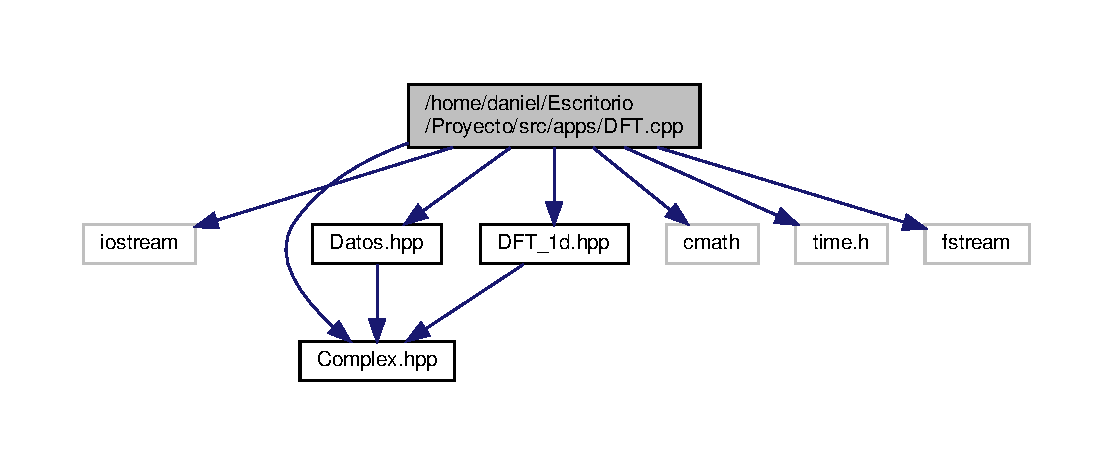
\includegraphics[width=350pt]{DFT_8cpp__incl}
\end{center}
\end{figure}
\subsection*{Functions}
\begin{DoxyCompactItemize}
\item 
\mbox{\Hypertarget{DFT_8cpp_ae66f6b31b5ad750f1fe042a706a4e3d4}\label{DFT_8cpp_ae66f6b31b5ad750f1fe042a706a4e3d4}} 
int {\bfseries main} ()
\end{DoxyCompactItemize}


\subsection{Detailed Description}
Algoritmo para obtener el tiempo de calculo de D\+FT. 

Hallar el tiempo demorado para calcular la D\+FT de distintos tamaños de arrays. \begin{DoxyAuthor}{Author}
Daniel Reyes Barrera 
\end{DoxyAuthor}
\begin{DoxyVersion}{Version}
1.\+0 
\end{DoxyVersion}
\begin{DoxyDate}{Date}
2021 
\end{DoxyDate}
\begin{DoxyCopyright}{Copyright}
G\+NU Public License. 
\end{DoxyCopyright}

\hypertarget{FFT_8cpp}{}\section{/home/daniel/\+Escritorio/\+Proyecto/src/apps/\+F\+FT.cpp File Reference}
\label{FFT_8cpp}\index{/home/daniel/\+Escritorio/\+Proyecto/src/apps/\+F\+F\+T.\+cpp@{/home/daniel/\+Escritorio/\+Proyecto/src/apps/\+F\+F\+T.\+cpp}}


Algoritmo para obtener el tiempo de calculo de F\+FT.  


{\ttfamily \#include $<$cmath$>$}\newline
{\ttfamily \#include $<$Complex.\+hpp$>$}\newline
{\ttfamily \#include $<$Datos.\+hpp$>$}\newline
{\ttfamily \#include $<$F\+F\+T\+\_\+1d.\+hpp$>$}\newline
{\ttfamily \#include $<$iostream$>$}\newline
{\ttfamily \#include $<$time.\+h$>$}\newline
{\ttfamily \#include $<$fstream$>$}\newline
Include dependency graph for F\+F\+T.\+cpp\+:
\nopagebreak
\begin{figure}[H]
\begin{center}
\leavevmode
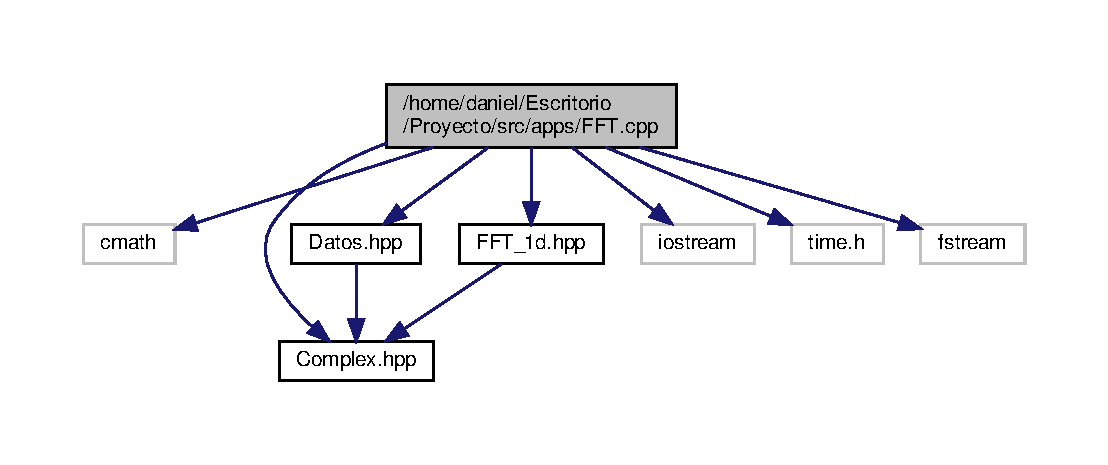
\includegraphics[width=350pt]{FFT_8cpp__incl}
\end{center}
\end{figure}
\subsection*{Functions}
\begin{DoxyCompactItemize}
\item 
\mbox{\Hypertarget{FFT_8cpp_ae66f6b31b5ad750f1fe042a706a4e3d4}\label{FFT_8cpp_ae66f6b31b5ad750f1fe042a706a4e3d4}} 
int {\bfseries main} ()
\end{DoxyCompactItemize}


\subsection{Detailed Description}
Algoritmo para obtener el tiempo de calculo de F\+FT. 

Hallar el tiempo demorado para calcular la F\+FT de distintos tamaños de arrays. \begin{DoxyAuthor}{Author}
Daniel Reyes Barrera 
\end{DoxyAuthor}
\begin{DoxyVersion}{Version}
1.\+0 
\end{DoxyVersion}
\begin{DoxyDate}{Date}
2021 
\end{DoxyDate}
\begin{DoxyCopyright}{Copyright}
G\+NU Public License. 
\end{DoxyCopyright}

\hypertarget{Complex_8hpp}{}\section{/home/daniel/\+Escritorio/\+Proyecto/src/lib/include/\+Complex.hpp File Reference}
\label{Complex_8hpp}\index{/home/daniel/\+Escritorio/\+Proyecto/src/lib/include/\+Complex.\+hpp@{/home/daniel/\+Escritorio/\+Proyecto/src/lib/include/\+Complex.\+hpp}}


Clase para almacenar datos tipo complejos.  


This graph shows which files directly or indirectly include this file\+:
\nopagebreak
\begin{figure}[H]
\begin{center}
\leavevmode
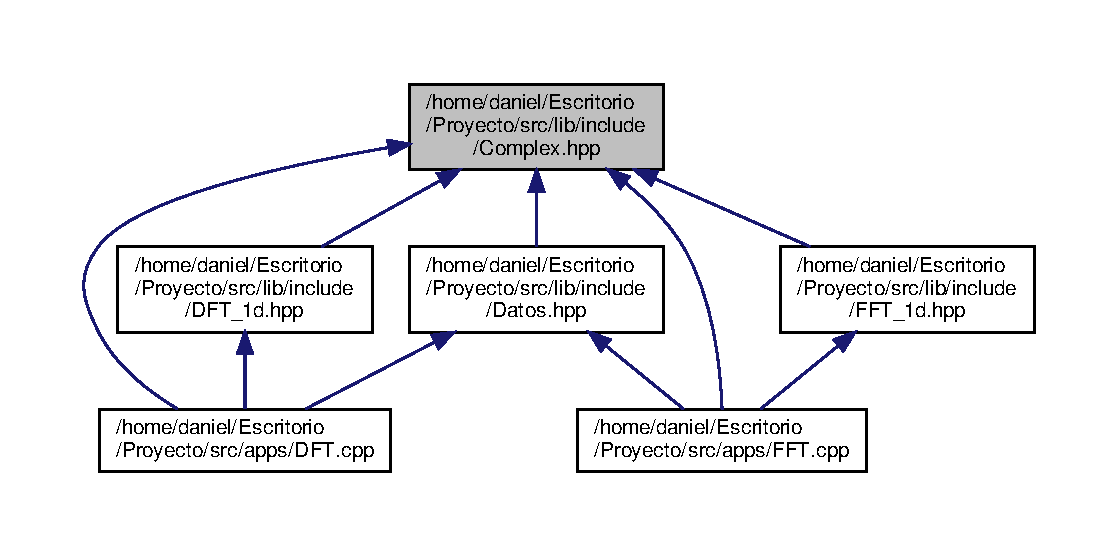
\includegraphics[width=350pt]{Complex_8hpp__dep__incl}
\end{center}
\end{figure}
\subsection*{Classes}
\begin{DoxyCompactItemize}
\item 
class \hyperlink{classComplex}{Complex}
\begin{DoxyCompactList}\small\item\em Clase \hyperlink{classComplex}{Complex}. \end{DoxyCompactList}\end{DoxyCompactItemize}


\subsection{Detailed Description}
Clase para almacenar datos tipo complejos. 

Una clase simple que contine dos variables tipo double. \begin{DoxyAuthor}{Author}
Daniel Reyes Barrera 
\end{DoxyAuthor}
\begin{DoxyVersion}{Version}
1.\+0 
\end{DoxyVersion}
\begin{DoxyDate}{Date}
2021 
\end{DoxyDate}
\begin{DoxyCopyright}{Copyright}
G\+NU Public License. 
\end{DoxyCopyright}

\hypertarget{Datos_8hpp}{}\section{/home/daniel/\+Escritorio/\+Proyecto/src/lib/include/\+Datos.hpp File Reference}
\label{Datos_8hpp}\index{/home/daniel/\+Escritorio/\+Proyecto/src/lib/include/\+Datos.\+hpp@{/home/daniel/\+Escritorio/\+Proyecto/src/lib/include/\+Datos.\+hpp}}


Clase para obtener y manipular los datos de entrada para los algoritmos.  


{\ttfamily \#include $<$Complex.\+hpp$>$}\newline
Include dependency graph for Datos.\+hpp\+:
\nopagebreak
\begin{figure}[H]
\begin{center}
\leavevmode
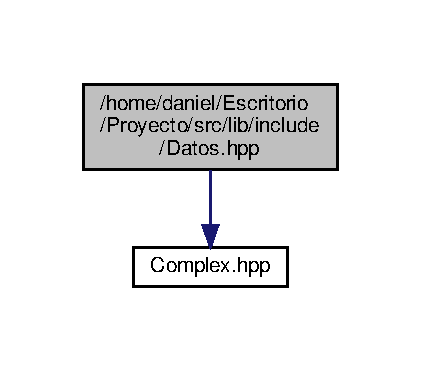
\includegraphics[width=202pt]{Datos_8hpp__incl}
\end{center}
\end{figure}
This graph shows which files directly or indirectly include this file\+:
\nopagebreak
\begin{figure}[H]
\begin{center}
\leavevmode
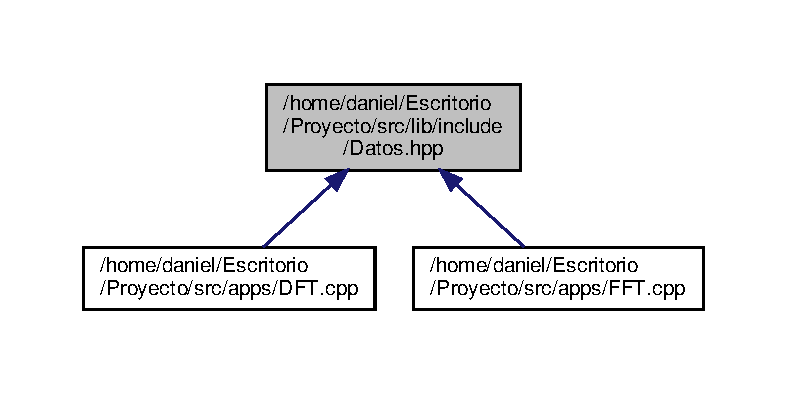
\includegraphics[width=350pt]{Datos_8hpp__dep__incl}
\end{center}
\end{figure}
\subsection*{Classes}
\begin{DoxyCompactItemize}
\item 
class \hyperlink{classDatos}{Datos}
\begin{DoxyCompactList}\small\item\em Clase \hyperlink{classDatos}{Datos}. \end{DoxyCompactList}\end{DoxyCompactItemize}


\subsection{Detailed Description}
Clase para obtener y manipular los datos de entrada para los algoritmos. 

Una clase que contiene varios metodos para la obtencion y manipulacion de datos. \begin{DoxyAuthor}{Author}
Daniel Reyes Barrera 
\end{DoxyAuthor}
\begin{DoxyVersion}{Version}
1.\+0 
\end{DoxyVersion}
\begin{DoxyDate}{Date}
2021 
\end{DoxyDate}
\begin{DoxyCopyright}{Copyright}
G\+NU Public License. 
\end{DoxyCopyright}

\hypertarget{DFT__1d_8hpp}{}\section{/home/daniel/\+Escritorio/\+Proyecto/src/lib/include/\+D\+F\+T\+\_\+1d.hpp File Reference}
\label{DFT__1d_8hpp}\index{/home/daniel/\+Escritorio/\+Proyecto/src/lib/include/\+D\+F\+T\+\_\+1d.\+hpp@{/home/daniel/\+Escritorio/\+Proyecto/src/lib/include/\+D\+F\+T\+\_\+1d.\+hpp}}


Clase para calcular la D\+FT.  


{\ttfamily \#include $<$Complex.\+hpp$>$}\newline
Include dependency graph for D\+F\+T\+\_\+1d.\+hpp\+:
\nopagebreak
\begin{figure}[H]
\begin{center}
\leavevmode
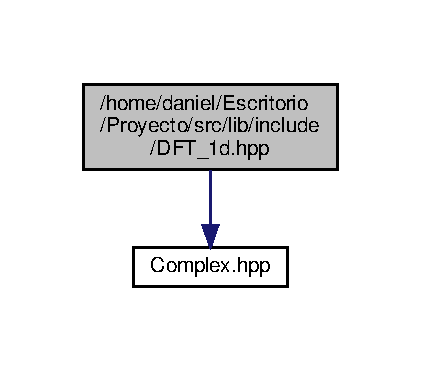
\includegraphics[width=202pt]{DFT__1d_8hpp__incl}
\end{center}
\end{figure}
This graph shows which files directly or indirectly include this file\+:
\nopagebreak
\begin{figure}[H]
\begin{center}
\leavevmode
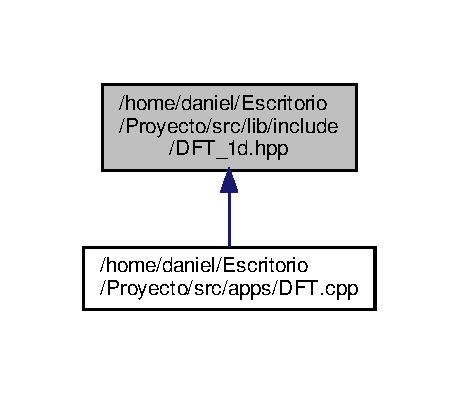
\includegraphics[width=220pt]{DFT__1d_8hpp__dep__incl}
\end{center}
\end{figure}
\subsection*{Classes}
\begin{DoxyCompactItemize}
\item 
class \hyperlink{classDFT__1d}{D\+F\+T\+\_\+1d}
\begin{DoxyCompactList}\small\item\em Clase \hyperlink{classDFT__1d}{D\+F\+T\+\_\+1d}. \end{DoxyCompactList}\end{DoxyCompactItemize}


\subsection{Detailed Description}
Clase para calcular la D\+FT. 

Una clase que contiene un metodo para calcular la D\+FT de un array. \begin{DoxyAuthor}{Author}
Daniel Reyes Barrera 
\end{DoxyAuthor}
\begin{DoxyVersion}{Version}
1.\+0 
\end{DoxyVersion}
\begin{DoxyDate}{Date}
2021 
\end{DoxyDate}
\begin{DoxyCopyright}{Copyright}
G\+NU Public License. 
\end{DoxyCopyright}

\hypertarget{FFT__1d_8hpp}{}\section{/home/daniel/\+Escritorio/\+Proyecto/src/lib/include/\+F\+F\+T\+\_\+1d.hpp File Reference}
\label{FFT__1d_8hpp}\index{/home/daniel/\+Escritorio/\+Proyecto/src/lib/include/\+F\+F\+T\+\_\+1d.\+hpp@{/home/daniel/\+Escritorio/\+Proyecto/src/lib/include/\+F\+F\+T\+\_\+1d.\+hpp}}


Clase para calcular la F\+FT.  


{\ttfamily \#include $<$Complex.\+hpp$>$}\newline
Include dependency graph for F\+F\+T\+\_\+1d.\+hpp\+:
\nopagebreak
\begin{figure}[H]
\begin{center}
\leavevmode
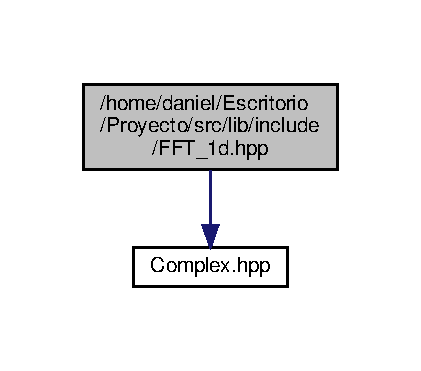
\includegraphics[width=202pt]{FFT__1d_8hpp__incl}
\end{center}
\end{figure}
This graph shows which files directly or indirectly include this file\+:
\nopagebreak
\begin{figure}[H]
\begin{center}
\leavevmode
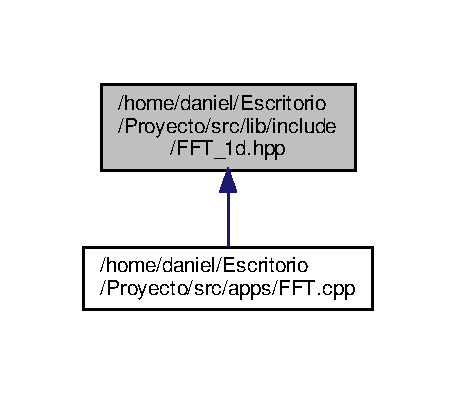
\includegraphics[width=219pt]{FFT__1d_8hpp__dep__incl}
\end{center}
\end{figure}
\subsection*{Classes}
\begin{DoxyCompactItemize}
\item 
class \hyperlink{classFFT__1d}{F\+F\+T\+\_\+1d}
\begin{DoxyCompactList}\small\item\em Clase \hyperlink{classFFT__1d}{F\+F\+T\+\_\+1d}. \end{DoxyCompactList}\end{DoxyCompactItemize}


\subsection{Detailed Description}
Clase para calcular la F\+FT. 

Una clase que contiene un metodo para calcular la F\+FT de un array. \begin{DoxyAuthor}{Author}
Daniel Reyes Barrera 
\end{DoxyAuthor}
\begin{DoxyVersion}{Version}
1.\+0 
\end{DoxyVersion}
\begin{DoxyDate}{Date}
2021 
\end{DoxyDate}
\begin{DoxyCopyright}{Copyright}
G\+NU Public License. 
\end{DoxyCopyright}

%--- End generated contents ---

% Index
\backmatter
\newpage
\phantomsection
\clearemptydoublepage
\addcontentsline{toc}{chapter}{Index}
\printindex

\end{document}
